\documentclass[sigplan,10pt]{acmart}\settopmatter{printfolios=true}
%% For final camera-ready submission
%\documentclass[sigplan,10pt]{acmart}\settopmatter{}

\settopmatter{printacmref=false} % Removes citation information below abstract
\renewcommand\footnotetextcopyrightpermission[1]{} % removes footnote with conference information in first column
\pagestyle{plain} % removes running headers

%% Some recommended packages.
\usepackage{booktabs}   %% For formal tables:
                        %% http://ctan.org/pkg/booktabs
\usepackage{subcaption} %% For complex figures with subfigures/subcaptions
                        %% http://ctan.org/pkg/subcaption

\usepackage{mathpartir}
\usepackage{xspace}
\usepackage{stmaryrd}
\usepackage{listings}
\usepackage{newtxmath}

%% Tikz Needed packages
\usepackage{pgfplots}
\pgfplotsset{width=7cm,compat=1.8}
\usepackage{pgfplotstable}
\renewcommand*{\familydefault}{\sfdefault}


\makeatletter\if@ACM@journal\makeatother
%% Journal information (used by PACMPL format)
%% Supplied to authors by publisher for camera-ready submission
\acmJournal{ICFP 17 student research competition}
\acmVolume{1}
\acmNumber{1}
\acmArticle{1}
\acmYear{2017}
\acmMonth{1}
\acmDOI{10.1145/nnnnnnn.nnnnnnn}
\startPage{1}
\else\makeatother
%% Conference information (used by SIGPLAN proceedings format)
%% Supplied to authors by publisher for camera-ready submission
\acmConference[ICFP 2017 Student Research Competition]{ICFP 2017 Student Research Competition}{September, 2017}{Oxford, UK}
\acmYear{2017}
\acmISBN{978-x-xxxx-xxxx-x/YY/MM}
\acmDOI{10.1145/nnnnnnn.nnnnnnn}
\startPage{1}
\fi

%% Copyright information
%% Supplied to authors (based on authors' rights management selection;
%% see authors.acm.org) by publisher for camera-ready submission
\setcopyright{none}             %% For review submission
%\setcopyright{acmcopyright}
%\setcopyright{acmlicensed}
%\setcopyright{rightsretained}
%\copyrightyear{2017}           %% If different from \acmYear

%% Bibliography style
\bibliographystyle{ACM-Reference-Format}
%% Citation style
%% Note: author/year citations are required for papers published as an
%% issue of PACMPL.
%\citestyle{acmauthoryear}  %% For author/year citations
%\citestyle{acmnumeric}     %% For numeric citations
%\setcitestyle{nosort}      %% With 'acmnumeric', to disable automatic
                            %% sorting of references within a single citation;
                            %% e.g., \cite{Smith99,Carpenter05,Baker12}
                            %% rendered as [14,5,2] rather than [2,5,14].
%\setcitesyle{nocompress}   %% With 'acmnumeric', to disable automatic
                            %% compression of sequential references within a
                            %% single citation;
                            %% e.g., \cite{Baker12,Baker14,Baker16}
                            %% rendered as [2,3,4] rather than [2-4].

\newcommand{\lang}{\textsc{Effy}\xspace}
\newcommand{\eff}{\textsc{Eff}\xspace}
\newcommand{\ocaml}{\textsc{OCaml}\xspace}

% Meta-syntax
\newcommand{\bnfis}{\mathrel{\;{:}{:}\!=}\;}
\newcommand{\bnfor}{\mathrel{\;|\;}}
\newcommand{\defeq}{\mathrel{\;\stackrel{\text{def}}{=}\;}}
\newcommand{\set}[1]{\{ #1 \}}

% General syntactic constructs
\newcommand{\kord}[1]{\mathtt{#1}}
\newcommand{\kop}[1]{\;\mathtt{#1}\;}
\newcommand{\kpre}[1]{\mathtt{#1}\;}
\newcommand{\kpost}[1]{\;\mathtt{#1}}

% Types
\newcommand{\type}[1]{\mathtt{#1}}
\newcommand{\boolty}{\type{bool}}
\newcommand{\intty}{\type{int}}
\newcommand{\hto}{\Rightarrow}
\renewcommand{\C}{\underline{C}}
\newcommand{\D}{\underline{D}}
\newcommand{\dirt}{\Delta}
\newcommand{\sig}{\Sigma}

% Expressions and computations
\newcommand{\funtyped}[2]{\kpre{fun} #1 \T #2 \mapsto}

\newcommand{\call}[3]{{{#1}\,{#2}\,{#3}}}
\newcommand{\case}{\mathop{\text{\texttt{|}}}}
\newcommand{\cont}[2]{(#1.\,#2)}
\newcommand{\const}{\kord{k}}
\newcommand{\fls}{\kord{false}}
\newcommand{\fun}[1]{\kpre{fun} #1 \mapsto}
\newcommand{\handler}[1]{\{ #1 \}}
\newcommand{\conditional}[3]{\kpre{if} #1 \kop{then} #2 \kop{else} #3}
\newcommand{\letin}[1]{\kpre{let} #1 \kop{in}}
\newcommand{\doin}[1]{\kpre{do} #1 \kop{ ; }}
\newcommand{\letrecin}[1]{\kpre{let} \kpre{rec} #1 \kop{in}}
\newcommand{\op}{\kord{Op}}
\newcommand{\ops}{\mathcal{O}}
\newcommand{\ocs}{\mathit{ocs}}
\newcommand{\ocsnil}{\kord{nil}}
\newcommand{\tru}{\kord{true}}
\newcommand{\ret}{\kpre{return}}
\newcommand{\withhandle}[2]{\kpre{handle} #2 \kop{with} #1}
\newcommand{\pure}[1]{\kord{pure } #1  }
\newcommand{\longcases}{\call{\op_1}{y}{k} \mapsto c_{\op_1}, \ldots, \call{\op_n}{x}{k} \mapsto c_{\op_n}}
\newcommand{\shortcases}{[\call{\op}{y}{k} \mapsto c_\op]_{\op \in \ops}}
\newcommand{\longhand}[1][\ret x \mapsto c_r]{\handler{#1, \longcases}}
\newcommand{\shorthand}[1][\ret x \mapsto c_r]{\handler{#1, \shortcases}}

% Type-checking
\newcommand{\row}{\mathrel{;} R}
\newcommand{\ctx}{\Gamma}
\newcommand{\ent}{\vdash}
\newcommand{\T}{\mathrel{:}}
\newcommand{\E}{\mathrel{!}}
\newcommand{\covers}{\mathrel{/}}
\renewcommand{\le}{\leqslant}

% Operational semantics
\newcommand{\eval}{\Downarrow}
\newcommand{\hs}{\mathcal{H}}
\newcommand{\nil}{\emptyset}
\newcommand{\cons}{\mathbin{::}}
\newcommand{\hseval}[1][\hs]{\Downarrow_{#1}}
\newcommand{\getval}[1]{{#1}_{\kord{val}}}
\newcommand{\getop}[1]{{#1}_{\kord{op}}}

\newcommand{\todo}[1]{\textcolor{red}{\textsc{Todo:} #1}}

\begin{document}

\title{Towards a core language with row-based effects for optimised compilation}

\author{Axel Faes}
\affiliation{
  \position{student : undergraduate\\ACM Student Member: 2461936}
  \department{Department of Computer Science}
  \institution{KU Leuven}
}
\email{axel.faes@student.kuleuven.be}

\author{Tom Schrijvers}
\affiliation{
  \position{advisor}
  \department{Department of Computer Science}
  \institution{KU Leuven}
}
\email{tom.schrijvers@kuleuven.be}

%% Keywords
%% comma separated list
\keywords{algebraic effect handler, row based effect, optimised compilation}  %% \keywords is optional

%% Abstract
%% Note: \begin{abstract}...\end{abstract} environment must come
%% before \maketitle command
\begin{abstract}
Algebraic effects and handlers are a very active area of research. An important aspect is the development of an optimising compiler. \eff is an ML-style language with support for effects and forms the testbed for the optimising compiler. However, \eff does not offer explicit typing, which makes it easy for type checking bugs to be introduced during the construction of optimised compilation. This work presents a new core language with row-based effects. The core language is explicitly typed in order to reduce bugs in the optimised compilation.
\end{abstract}

\maketitle

\section{Introduction}
\label{intro}
Algebraic effect handling is a very active area of research. Implementations of algebraic effect handlers are becoming available. Because of this, improving performance is becoming the focus of research. A lot of research focusses on speeding up the runtime performance. However, a runtime penalty still occurs. This happens since handlers or continuations need to be repeatedly copied on the heap. Due to this, we are looking towards type-directed optimised compilation of algebraic effect handlers. We want to remove the handlers such that no copying is required and thus no runtime penalty occurs. \\
\\
In our ongoing research towards type-directed optimised compilation, term rewrite rules and purity aware compilation optimise away most handlers. Term rewrite rules use information of the type-\&-effect system. Term rewrite rules perform two types of actions. They remove handlers and apply effects such that eventually the program does not contain any more handlers. Term rewrite rules can also change the syntactic structure in order to expose more possibilities for optimisations. Purity aware compilation identifies computations that are effectively pure and purifies them.  \\
\\
\eff, an ML-style language, is being used to develop an optimised compiler for algebraic effect handlers. \eff uses a type system based on subtyping \cite{effectsystem}. As explained by Bauer and Pretnar in \cite{programming}, terms in \eff do not contain any information about computational effects. This information has to be inferred using type inference algorithms. The lack of explicit type information makes source-to-source transformations much more error-prone. Additionally, ensuring that a transformation does not break typeability becomes a time-consuming task, since we need to reconstruct types after each optimisation pass. \\
\\
The current type system with subtyping becomes impractical since the typing information is not explicitly contained in each term. There are several solutions to make the type system more practical. It is possible to keep subtyping, but use a unification based algorithm \cite{mlsub}. Implicit effect polymorphism can also be used \cite{impliciteff}. The option that is explored in this work, is to use a simple type-\&-effect system based on row-polymorphism \cite{type-directed, leijen2014koka, row}. \\
\\
In this work, we present a simple explicitly-typed language that can serve as an intermediate language during compilation of \eff, and allows for the development of type-preserving core-to-core transformations. Optimisation and term rewriting is done using this core language. This approach will ease the development of an optimised compiler since typechecking becomes linear due to the explicit typing.

\section{Background}
The type-\&-effect system that is used in \eff is based on subtyping and dirty types \cite{effectsystem}.

\paragraph{Terms}
Figure~\ref{fig:terms:eff} shows the two types of terms in \eff. There are values $v$ and computations $c$. Computations are terms that can contain effects. Effects are denoted as operations $Op$ which can be called.

\paragraph{Types}
Figure~\ref{fig:types:eff} shows the types of \eff. There are two main sorts of types. There are (pure) types $A, B$ and dirty types $\C, \D$. A dirty type is a pure type $A$ tagged with a finite set of operations $\dirt$, which we call dirt, that can be called. The type $\C \hto \D$ is used for handlers because a handler takes an input computation $\C$, handles the effects in this computation and outputs computation $\D$ as the result.\\
\\
The core language with row-based effects is based on the explicitly typed language used in Links \cite{row}. Links uses a row polymorphic type-\&-effect system . The design of their calculus is partially based on the type system used by Pretnar which makes it a suitable candidate for our core language \cite{pretnar2015introduction}. The terms of the core language are seen in Figure~\ref{fig:terms:explicit}, the types are seen in the Figure~\ref{fig:types:explicit}.

\begin{figure}[h]
\begin{center}
\framebox{
\begin{minipage}{0.98\columnwidth}
\[\begin{array}{r@{~}c@{~}l@{\quad}l}
  \text{value}~v & \bnfis {} & x & \text{variable} \\
    & \bnfor & \const & \text{constant} \\
    & \bnfor & \fun{x} c & \text{function} \\
    & \bnfor & \{ & \text{handler} \\
    & & \quad \ret x \mapsto c_r, & \quad\text{return case} \\
    & & \quad \shortcases & \quad\text{operation cases} \\
    & & \} & \\
  \text{comp}~c & \bnfis & v_1 \, v_2 & \text{application} \\
    & \bnfor & \letrecin{f \, x = c_1} c_2 & \text{rec definition} \\
    & \bnfor & \ret v  & \text{returned val} \\
    & \bnfor & \op \, v & \text{operation call} \\
    & \bnfor & \doin{x \leftarrow c_1} c_2 & \text{sequencing} \\
    & \bnfor & \withhandle{v}{c} & \text{handling}
\end{array}\]
\end{minipage}
}
\end{center}
\caption{Terms of \eff as described in previous work}\label{fig:terms:eff}
\end{figure}
\begin{figure}
\begin{center}
\framebox{
\begin{minipage}{0.98\columnwidth}
\[\begin{array}{r@{~}c@{~}l@{\quad}l}
  \text{(pure) type}~A, B & \bnfis {}
    & \boolty \bnfor \intty & \text{basic types} \\
    & \bnfor & A \to \C & \text{function type} \\
    & \bnfor & \C \hto \D & \text{handler type} \\
  \text{dirty type}~\C, \D & \bnfis {} & A \E \dirt \\
  \text{dirt}~\dirt & \bnfis {} &\set{\op_1, \dots, \op_n}
\end{array}\]
\end{minipage}
}
\end{center}
\caption{Types of \eff as described in previous work}\label{fig:types:eff}
\end{figure}

\begin{figure}[h]
\begin{center}
\framebox{
\begin{minipage}{0.98\columnwidth}
\[\begin{array}{r@{~}c@{~}l@{\quad}l}
  \text{value}~v & \bnfis {} & x & \text{variable} \\
    & \bnfor & \const & \text{constant} \\
    & \bnfor & \lambda (x : A). c & \text{\textbf{function}} \\
    & \bnfor & \Lambda \alpha . c & \text{\textbf{type abstraction}} \\
    & \bnfor & \{ & \text{handler} \\
    & & \quad \ret x \mapsto c_r, & \quad\text{return case} \\
    & & \quad \shortcases & \quad\text{operation cases} \\
    & & \} & \\
  \text{comp}~c & \bnfis & v_1 \, v_2 & \text{application} \\
    & \bnfor & v \, A & \text{\textbf{type application}} \\
    & \bnfor & \letrecin{f \, x = c_1} c_2 & \text{rec definition} \\
    & \bnfor & \ret v  & \text{returned val} \\
    & \bnfor & \op \, v & \text{operation call} \\
    & \bnfor & \doin{x \leftarrow c_1} c_2 & \text{sequencing} \\
    & \bnfor & \withhandle{v}{c} & \text{handling}
\end{array}\]
\end{minipage}
}
\end{center}
\caption{Terms of the explicitly typed core language}\label{fig:terms:explicit}
\end{figure}

\begin{figure}
\begin{center}
\framebox{
\begin{minipage}{0.98\columnwidth}
\[\begin{array}{r@{~}c@{~}l@{\quad}l}
  \text{(pure) type}~A, B & \bnfis {}
    & A \to \C & \text{function type} \\
    & \bnfor & \C \hto \D & \text{handler type} \\
    & \bnfor & \alpha & \text{\textbf{type variable}} \\
    & \bnfor & \forall \alpha . \C & \text{\textbf{polytype}} \\
  \text{dirty type}~\C, \D & \bnfis {} & A \E \dirt \\
  \text{dirt}~\dirt & \bnfis {} &\set{\op_1, \dots, \op_n}
\end{array}\]
\end{minipage}
}
\end{center}
\caption{Types of the explicitly type core language}\label{fig:types:explicit}
\end{figure}

%\section{Approach and Uniqueness}
\section{Results and Contributions}
Preliminary results show that optimised compilation of \eff reaches the same performance as an implementation without algebraic effect handlers in OCaml (Figure~\ref{fig:systemsall}). Unfortunately, the development of several optimisations proved to be very error-prone, illustrating the need for an explicitly-typed core language. \\
\\
The proposed core language with row-based effects makes it easier to develop an optimised compiler due to the explicit typing. Since \eff focusses on ease-of-use and usability, the programmer will not be burdened with providing more type information than minimally required \cite{inferring, handling}. The combination of these languages gives the best of both worlds.
\\
\begin{figure}
  \resizebox{\columnwidth}{!}{%
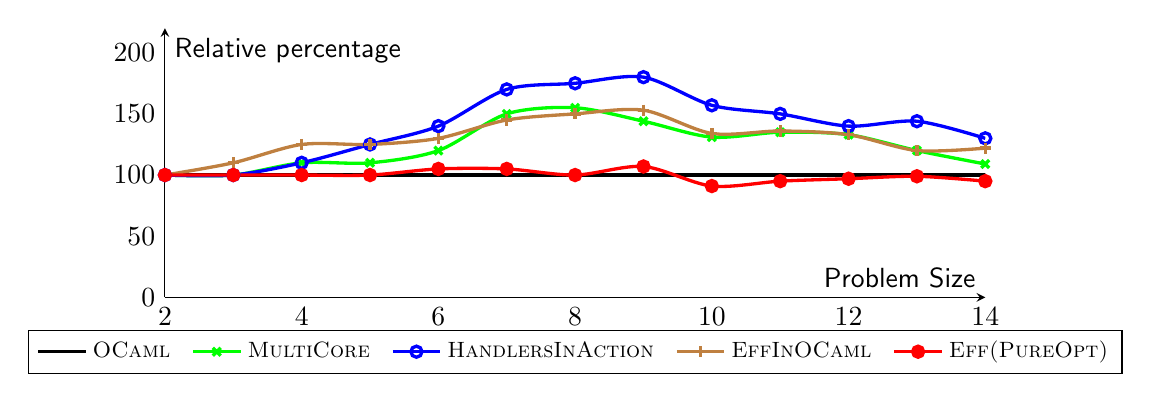
\begin{tikzpicture}
  \centering
  \begin{axis}[
        axis lines=center,
        axis on top,
        height=5cm, width=12cm,
        % bar width=0.4cm,
        % ymajorgrids, tick align=inside,
        major grid style={draw=white},
        enlarge y limits={value=.1,upper},
        ymin=0, ymax=200,
        axis x line*=bottom,
        axis y line*=left,
        % xtick = data,
        y axis line style={opacity=1},
        tickwidth=0pt,
        enlarge x limits=false,
        legend style={
            at={(0.5,-0.12)},
            anchor=north,
            legend columns=-1,
            /tikz/every even column/.append style={column sep=0.2cm},
            font = \footnotesize
        },
        ylabel={Relative percentage},
        xlabel={Problem Size},
           % symbolic x coords={
           % 0,
           % 8,
           % 9,
           % 10,
           % 11,
           % 12,
           % % 13,
           % % 14
           % },
       %      nodes near coords={
       %  \pgfmathprintnumber{\pgfplotspointmeta}
       % }
    ]
    %native
    \addplot [smooth,color = black, very thick] coordinates {
      (2,100)
      (3,100)
      (4,100)
      (5,100)
      (6,100)
      (7,100)
      (8,100)
      (9,100)
      (10,100)
      (11,100)
      (12,100)
      (13,100)
      (14,100)
       };
    %multicore
    \addplot [smooth,color = green, very thick, mark = x] coordinates {
      (2,100)
      (3,100)
      (4,110)
      (5,110)
      (6,120)
      (7,150)
      (8,155)
      (9,144)
      (10,131)
      (11,135)
      (12,133)
      (13,120)
      (14,109)
       };
    %HIA
   \addplot [smooth,color = blue, very thick, mark = o] coordinates {
      (2,100)
      (3,100)
      (4,110)
      (5,125)
      (6,140)
      (7,170)
      (8,175)
      (9,180)
      (10,157)
      (11,150)
      (12,140)
      (13,144)
      (14,130)
       };
    %EffectsinOcaml
   \addplot [smooth,color = brown, very thick, mark = +] coordinates {
      (2,100)
      (3,110)
      (4,125)
      (5,125)
      (6,130)
      (7,145)
      (8,150)
      (9,153)
      (10,134)
      (11,136)
      (12,133)
      (13,120)
      (14,122)
       };
    %PureOpt
   \addplot [smooth,color = red, very thick, mark = *] coordinates {
      (2,100)
      (3,100)
      (4,100)
      (5,100)
      (6,105)
      (7,105)
      (8,100)
      (9,107)
      (10,91)
      (11,95)
      (12,97)
      (13,99)
      (14,95)
       };

    \legend{\ocaml, \textsc{MultiCore}, \textsc{HandlersInAction}, \textsc{EffInOCaml}, \textsc{\eff}\textsc{(PureOpt)}}
  \end{axis}
  \end{tikzpicture}
  }
\caption{Results of running N-Queens for all solutions on multiple systems}
\label{fig:systemsall}
\end{figure}

\noindent In this work, we presented an idea of a core language for optimised compilation. Planned in future work is the implementation. We will integrate the presented core language in the optimising compiler for \eff and benchmark its impact. The metatheory of the core language is still under development. We will test the explicitly typed core language in other typing systems. As mentioned in this work, another interesting research direction is the development of an unification based algorithm for the subtyping based type-\&-effect system which we will also explore in future work.

%% Acknowledgments
\begin{acks}
  I would like to thank Amr Hany Saleh for his continuous guidance and help. I would also like to thank Matija Pretnar for his support during my research.
\end{acks}

\bibliography{main}

\end{document}
